\subsection*{Problema 14}

\textbf{Enunciado:} Calcular la integral:
\begin{align*}
I = \int \dfrac{\cos x \, dx}{1 + \sin x + \cos x}
\end{align*}

\textbf{Solución:} 
Utilizamos la sustitución universal de 
Weierstrass $z = \tan\left(\dfrac{x}{2}\right)$. 
Las identidades trigonométricas son:
\begin{align*}
\sin x &= \dfrac{2z}{1 + z^2}, \quad 
\cos x = \dfrac{1 - z^2}{1 + z^2}, \\
dx &= \dfrac{2 \, dz}{1 + z^2}
\end{align*}

Sustituyendo estas expresiones en la 
integral original, obtenemos:
\begin{align*}
I &= \int \dfrac{\dfrac{1 - z^2}{1 + z^2} 
\left(\dfrac{2 \, dz}{1 + z^2}\right)}
{1 + \dfrac{2z}{1 + z^2} + \dfrac{1 - z^2}{1 + z^2}}
\end{align*}

Simplificando el denominador común 
$(1 + z^2)$ en el integrando:
\begin{align*}
I &= \int \dfrac{2(1 - z^2) \, dz}
{(1 + z^2)(1 + z^2 + 2z + 1 - z^2)} \\
I &= \int \dfrac{2(1 - z^2) \, dz}
{(1 + z^2)(2 + 2z)}
\end{align*}

Cancelando el factor común $2$ y factorizando 
el denominador:
\begin{align*}
I &= \int \dfrac{(1 - z)(1 + z) \, dz}
{(1 + z^2)(1 + z)} = \int \dfrac{1 - z}{1 + z^2} \, dz
\end{align*}

Separando la integral en dos partes:
\begin{align*}
I &= \int \dfrac{1}{1 + z^2} \, dz - \int \dfrac{z}{1 + z^2} \, dz
\end{align*}

Resolviendo cada integral de forma directa:
\begin{align*}
I &= \arctan(z) - \dfrac{1}{2}\ln(1 + z^2) + C
\end{align*}

Regresando a la variable original $x$ 
mediante $z = \tan\left(\dfrac{x}{2}\right)$:
\begin{align*}
I &= \arctan\left(\tan\left(\dfrac{x}{2}\right)\right) \\
&\quad - \dfrac{1}{2}\ln\left(1 + \tan^2\left(\dfrac{x}{2}\right)\right) + C
\end{align*}

Simplificando usando identidades 
trigonométricas ($1 + \tan^2(\theta) = \sec^2(\theta)$):
\begin{align*}
I &= \dfrac{x}{2} - \dfrac{1}{2}\ln\left(\sec^2\left(\dfrac{x}{2}\right)\right) + C \\
I &= \dfrac{x}{2} - \ln\left|\sec\left(\dfrac{x}{2}\right)\right| + C
\end{align*}

\begin{figure}[H]
	\centering
	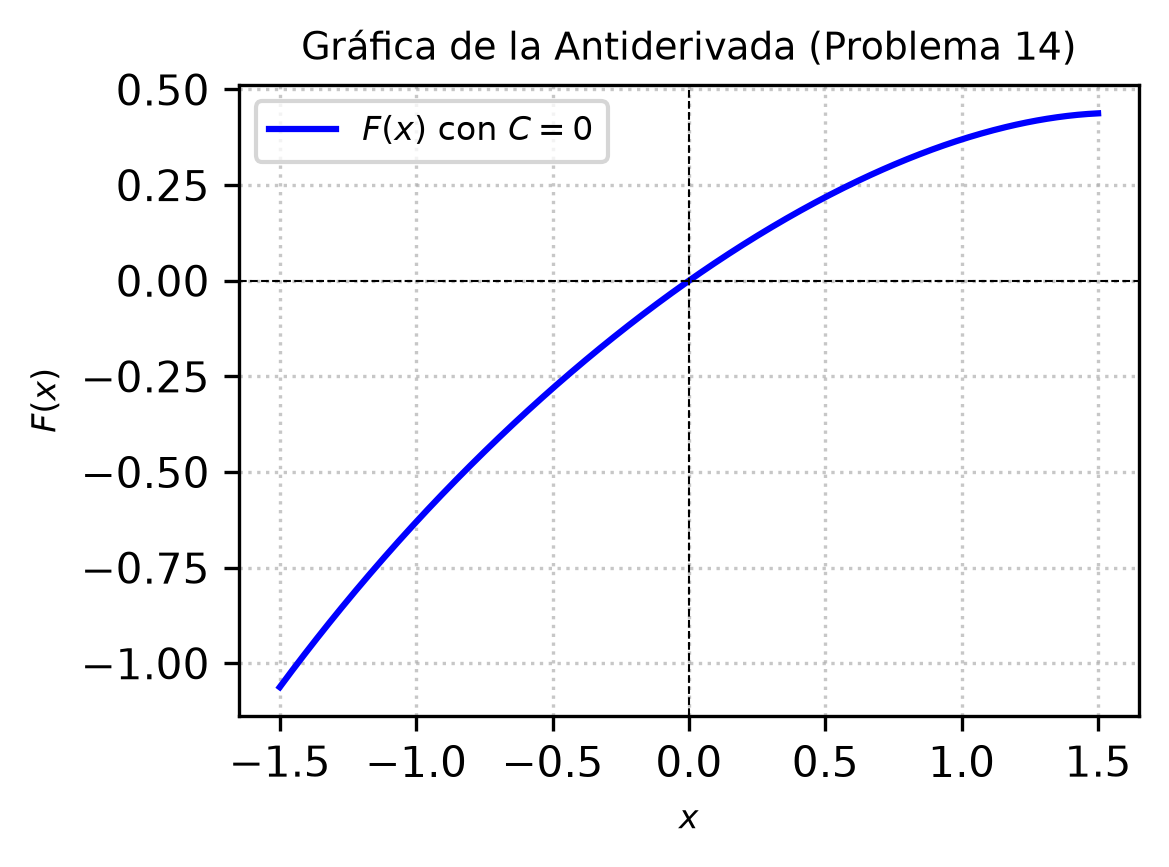
\includegraphics[width=\columnwidth]{semana_04/graficas/SEM04_P14_grafica.png}
	\caption{Representación gráfica de $f(x)$ y su antiderivada $F(x)$ evaluada para la constante de integración $C = 0$ (Problema 14).}
	\label{fig:problema14}
\end{figure}
